\part{A chacun sa culture qui fait rêver}
\chapter{Le Chili}

\chapter{Le Japon à travers les animes et les mangas}

\chapter{Le Japon : Matsuris et Croyances}
\section{Les croyances ...}
\paragraph{}
Le Japon ne possède pas de religion particulière. En effet, les japonais auront tendance à se considérer comme appartenant à aucune religion ou à plusieurs religions en même temps. Les religions principales sont le shintoïsme et le bouddhisme mais il y a une minorité de chrétiens et de musulmans. 
\paragraph{}
Ce mélange de religion est possible grâce aux caractéristiques des religions principales du pays. Le shintoïsme est une religion polythéiste tandis que le bouddhisme correspond plus à une philosophie de vie accompagnée de méditation.
\paragraph{}
« On dit souvent que le Japonais naît, grandit et s’amuse shinto, s’éduque confucéen, se marie chrétien, vit dans l’irréligion et meurt bouddhiste ». (Le Japon des Japonais par Philippe PONS et Pierre-François SOUYRI)

\section{... à l'origine des matsuris}
\paragraph{}
Le shintoïsme et le bouddhisme sont à l’origine de nombreuses fêtes traditionnelles autrement appelées Matsuri. En effet, pour attirer la bienveillance des dieux, chacun d’entre eux est prié et vénéré lors de rituel et de fête. Bien que les japonais ne croient pas vraiment en ces dieux, ils accomplissent ces rituels au cas où les dieux existeraient et retireraient leur bienveillance envers les japonais.
\paragraph{}
Ces fêtes ont lieu régulièrement tout au long de l’année. Au printemps, les Japonais fêtent le repiquage du riz et prient pour se protéger des épidémies. En été, ils prient pour se protéger contre les typhons et les ravages causés par les insectes ainsi que pour leurs ancêtres.  En hiver, ils prient pour la nouvelle année. Il y a aussi des fêtes locales pour prier les dieux locaux à différents moments de l’année. 
\paragraph{}
Lors de ces festivités, les hommes défilent dans le quartier en portant le mikoshi (sorte d’autel portatif) sur leurs dos. Ils sont vêtus d’un happi (veste découvrant leurs torses) et d’un fundoshi (sorte de cache-sexe traditionnel). Une fois l’autel retourné au temple, la fête continu le long de la rue du temple où l’on peut trouver des stands de friandises en sucres, de nouilles sautées, de porte-bonheurs… 
\begin{center}
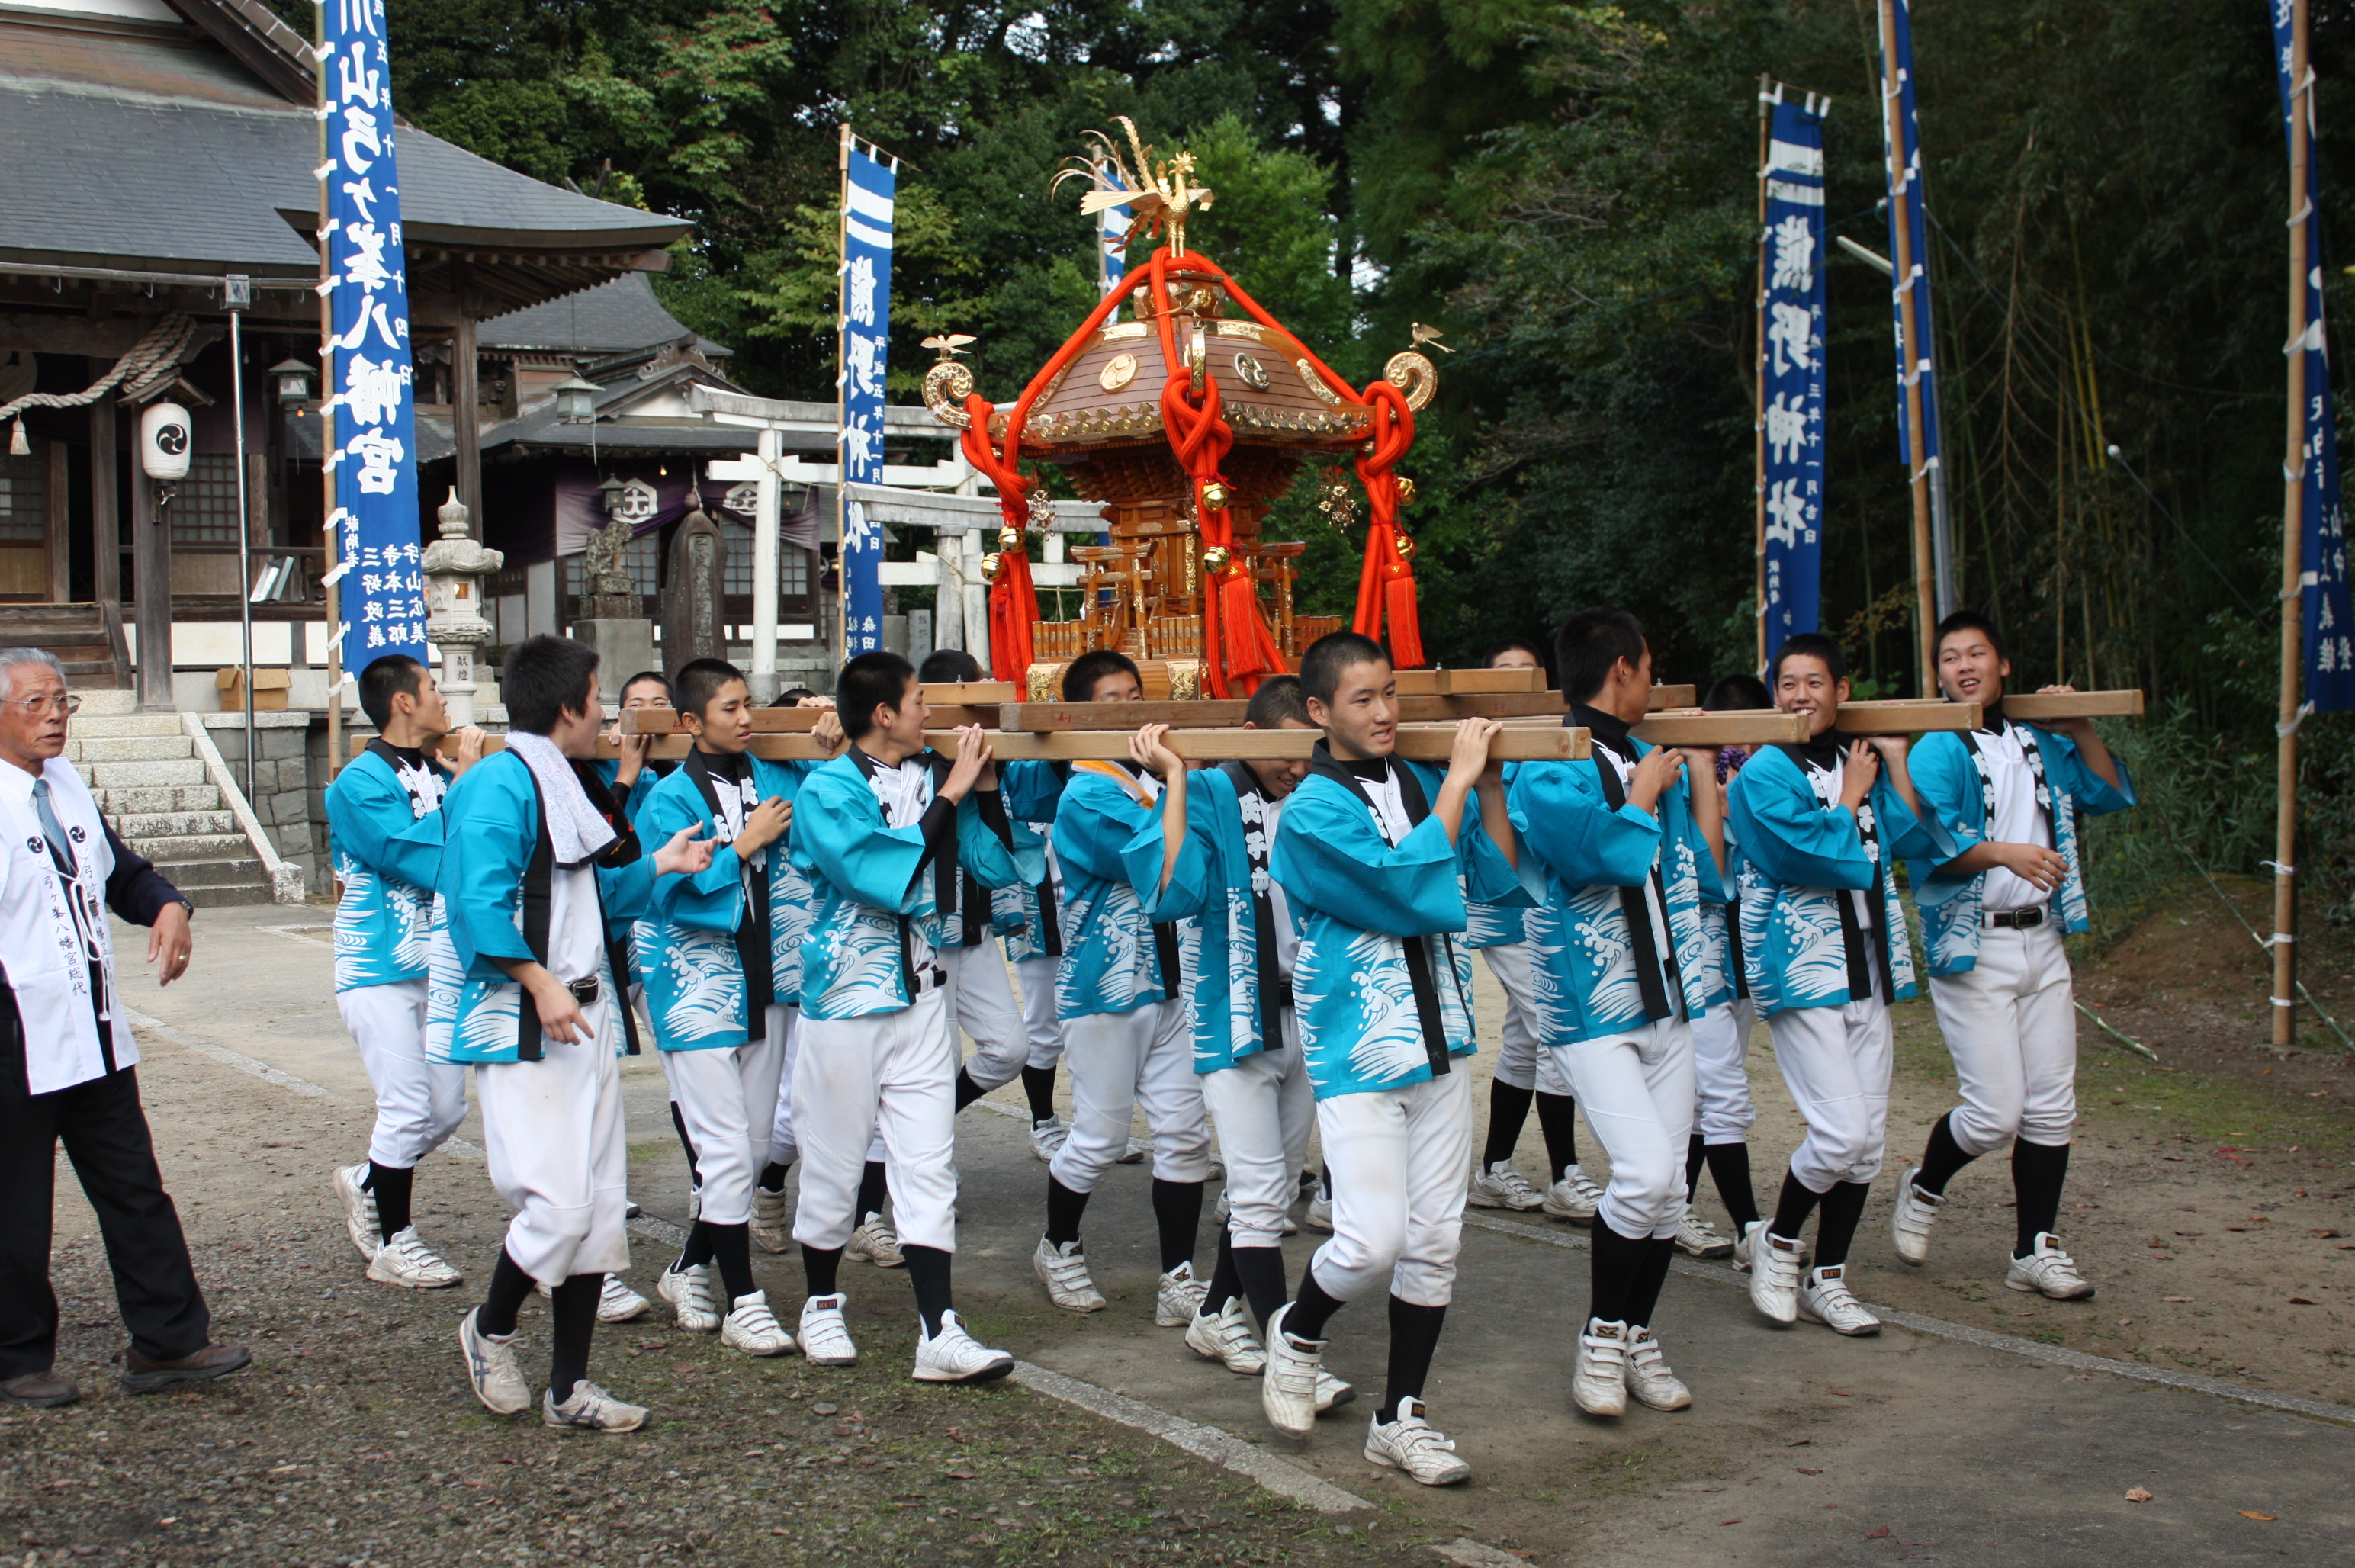
\includegraphics[scale=0.07]{mikoshi.jpg}
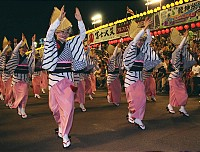
\includegraphics[scale=1.3]{odori.jpg}
\end{center}
\paragraph{}
Dans les plus grands matsuris, de grands chars défilent à travers le quartier accompagnés des flûtes, tambours et gongs. Ces chars sont aussi accompagnés de troupes de danseurs. Les filles profitent de ces festivals pour sortir leurs kimonos pour rentrer dans l’ambiance de la fête.
\begin{center}
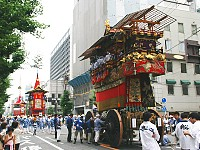
\includegraphics[scale=1.3]{gion.jpg}
\end{center}
\newpage
\section{Les matsuris les plus connus}
\begin{itemize}
\item Aoi matsuri, 15 mai, Kyoto
\item Aomori nebuta matsuri, 2-7 août, Aomori
\item Awa-Odori, 12-15 août, Tokushima
\item Danjiri matsuri, deuxième week end de septembre, Kishiwada
\item Etchu owara kaze no bon, 1-3 septembre Toyama
\item Gion matsuri, juillet, Kyoto quartier de Gion
\item Gozan no Okuribi, 16 août, Kyoto
\item Hadaka matsuri, troisième samedi de février, Okayama
\item Hakata Gion Yamakasa, 1-15 juillet, Hakata
\item Ise-jingu kannamesai et ninamesai, 15-25 octobre et 23-29 novembre, Ise
\item Jidai matsuri, 22 octobre, Kyoto
\item Kanda Matsuri, deuxième dimanche de mai, Tokyo
\item Namahage, 31 décembre, Oga
\item Narita-san setsubun-e, 3 février, Narita
\item Onbashira, avril tous les six ans, Suwa
\item Otaue matsuri, 14 juin, Osaka
\item Sanja matsuri, troisième week end de mai, Tokyo
\item Sanno matsuri, 14-15 avril, Takayama
\item Sendai Tanabata matsuri, 6-8 août, Sendai
\item Sentei-sai, 3-4 mai, Shimonoseki
\item Festival de la neige de Sapporo, mi-février, Sapporo
\item Tenjin matsuri, 24-25 juillet, Osaka
\item Yosakoi matsuri, 9-12 août, Kochi
\end{itemize}

\chapter{Les elfes}